\section{Durchführung}
\label{sec:Durchführung}
Damit die Funktionsweise und die Bedienung des Lasers geübt wird, werden verschiedene Messaufgaben durchgeführt.
%Der Laser ist so aufgebaut, dass über eine Stellschraube an der Seite der Reflexionswinkel des Gitters eingestellt werden kann.


\subsection{Bestimmen des Schwellenstroms}
\label{subsec:Schwellenstrom}
Für die Messung des Schwellenstroms, ab dem der Laser kohärentes Licht liefert, wird der Laser an eine Steuerelektronik angeschlossen. Mithilfe
dieser wird der Strom solange erhöht, bis auf einem Kamerabild einer Detektorkarte Lasergranulation zu beobachten ist. Die Detektorkarte reflektiert das Infrarotlicht
des Lasers so, dass es im optischen Spektrum liegt. Lasergranulation tritt aufgrund von Beugungseffekten des Lichtes an der mikroskopisch unebenen Oberfläche eines Materials auf
und ist an einem unregelmäßigen, fleckig gepunktetem Muster am Auftrittsort des Strahles zu erkennen.
Der Strom, ab dem gerade die Lasergranulation zu sehen ist, wird als der Schwellenstrom bezeichnet.


\subsection{Beobachten der Rubidiumfluoreszenz}
\label{subsec:Rubidiumfluoreszenz}
Wird der Laser auf eine Rubidiumzelle gerichtet, kann das Laserlicht das Rubidium soweit anregen, dass durch eine Kamera eine Fluoreszenz wahrzunehmen ist.
Dafür wird eine bestimmte Frequenz des Lichts benötigt, welche über Verstellen des Einstellwinkels des Gitters erreicht werden kann. Außerdem kann der an dem
Piezokristall anliegende Strom verändert werden, was zu Folge hat, dass dieser sein Volumen ändert, sodass auch hier die Frequenz des Laserlichts eingestellt
werden kann. Der Strom wird so eingestellt, dass er über dem Schwellenstrom liegt.


\subsection{Transmissionspektrum der Rubidiumzelle}
Damit das Transmissionspektrum der Rubidiumzelle aufgenommen werden kann, werden die Einstellungen des Lasers aus \ref{subsec:Rubidiumfluoreszenz} übernommen, der
Aufbau wird jedoch verändert. Zwischen der Rubidiumzelle und dem Laser wird ein 50/50-Strahlteiler installiert, der einen Teil des Strahls auf eine Photodiode lenkt.
Eine weitere Photodiode wird hinter der Rubidiumzelle aufgestellt. Über diese wird das tatsächliche Transmissionspektrum gemessen. Über einen Funktionsgenerator werden
die beiden Signale der Photodioden miteinander verrechnet, sodass ein Hintergrundrauschen herausgerechnet werden kann. Über ein Oszilloskop wird das bereinigte Signal
sichtbar gemacht.

\begin{figure}
    \centering
    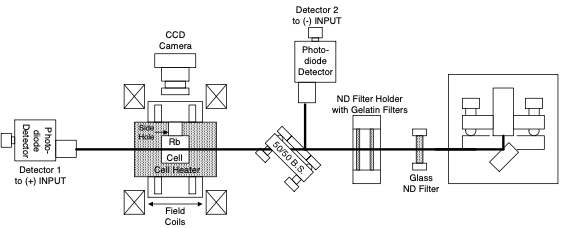
\includegraphics[width=\textwidth]{content/pics/Aufbau.png}
    \caption{Der verwendete Versuchsaufbau zur Bestimmung des Transmissionspektrums der Rubidiumzelle. \cite{diode_laser_spectroscopy}}
    \label{fig:Aufbau}
\end{figure}
